\section{Ice dynamics, the PISM view}\label{sec:dynamics}

\subsection{Two stress balance models: SIA and SSA}\index{PISM!SIA}\index{PISM!SSA}  At each time-step of a typical PISM run, the geometry, temperature, and basal strength of the ice sheet are included into stress (momentum) balance equations to determine the velocity of the flowing ice.   The ``full'' stress balance equations, namely the non-Newtonian Stokes model for slowly-flowing fluids \cite{Fowler}, are themselves the inertia-free approximation of the conservation of momentum equations.

PISM does not attempt to solve the Stokes equations themselves.  Instead it can numerically solve two different shallow approximations which are well-suited to ice sheet and ice shelf systems:
\begin{itemize}
\item the non-sliding shallow ice approximation (SIA)\index{SIA (shallow ice approximation)} \cite{Hutter}, also called the ``lubrication approximation'' \cite{Fowler}, which describes ice as flowing by shear in planes parallel to the geoid, with a strong contact of ice base to bedrock, and
\item the shallow shelf approximation (SSA)\index{SSA (shallow shelf approximation)} \cite{WeisGreveHutter}, which describes a membrane-type flow of floating ice \cite{Morland}, or of grounded ice which is sliding over a weak base \cite{MacAyeal,SchoofStream}.
\end{itemize}

PISM solves both the SIA and SSA equations in parallel.  The SIA\index{SIA (shallow ice approximation)!applicability} equations are easier to solve numerically than the SSA, and easier to parallelize, because they are local in each column of ice.\index{parallelization!relative ease of, between SIA and SSA}  Specifically, they describe the vertical shear stress as a local function of the driving stress \cite{Paterson}.  They can confidently be applied to those grounded parts of ice sheets for which the basal ice is frozen to the bedrock, or which is minimally sliding, and where the bed topography is relatively slowly-varying in the map-plane \cite{Fowler}.  These characteristics apply to the majority (by area) of the Greenland and Antarctic ice sheets.

We solve the SIA with a non-sliding base because the traditional \cite{Greve,HuybrechtsdeWolde,PayneBaldwin} addition of ad~hoc ``sliding laws''\index{SIA (shallow ice approximation)!sliding laws} into the SIA stress balance, and especially schemes which ``switch on'' at the pressure-melting temperature \cite{EISMINT00}, have bad continuum  \cite{Fowler01} and numerical \cite[appendix B]{BBssasliding} modeling consequences.

The SSA\index{SSA (shallow shelf approximation)!applicability} equations can confidently be applied to large floating ice shelves, which have small depth-to-width ratio and negligible basal resistance \cite{Morland,MorlandZainuddin}.  The flow speeds in ice shelves are frequently an order-of-magnitude higher than in the non-sliding, grounded parts of ice sheets.

Terrestrial ice sheets also have fast-flowing grounded parts, however, called ``ice streams'' or ``outlet glaciers'' \cite{TrufferEchelmeyer}.  Such features appear at the margin of, and sometimes well into the interior of, the Greenland \cite{Joughinetal2001}\index{Ice Sheets!Greenland ice sheet} and Antarctic \cite{BamberVaughanJoughin}\index{Ice Sheets!Antarctic ice sheet} ice sheets.  Describing these faster-flowing grounded parts of ice sheets requires something more than the non-sliding SIA.  This is because adjacent columns of ice which have different amounts of basal resistance exert strong ``longitudinal'' or ``membrane'' stresses \cite{SchoofStream} on each other.  One might use the Stokes equations, or a ``higher-order'' model (i.e.~less-shallow approximations \cite{Blatter,Pattyn03}), but this immediately leads to a resolution-versus-stress-inclusion tradeoff.  The amount of computation per map-plane grid location is much higher in higher-order models, although careful numerical analysis can generate large performance improvements for such equations \cite{BrownSmithAhmadia2013}.

As noted, both the SIA and SSA models are \emph{shallow} approximations.  These equations are derived from the Stokes equations by distinct small-parameter arguments, both based on a small depth-to-width ratio for the ice sheet.  For the small-parameter argument in the SIA case see \cite{Fowler}.  For the corresponding SSA argument, see \cite{WeisGreveHutter} or the appendices of \cite{SchoofStream}.  Schoof and Hindmarsh \cite{SchoofHindmarsh} have analyzed the connections between these shallowest models and higher-order models, while \cite{GreveBlatter2009} discusses ice dynamics and stress balances comprehensively.  Note that SIA, SSA, and higher-order models all approximate the pressure as hydrostatic.

With any membrane-stress-including model one must specify appropriate sliding boundary conditions.  The uncertainty in these boundary conditions usually dominate the modeling error made by not including higher-order stresses in the balance.  If the fast-flowing grounded ice is shallow (small aspect-ratio) then the SSA model can be applied, but a parameterized sliding relation must be chosen.  A well-known SSA model with a linear basal resistance relation is the Siple Coast (Antarctica) ice stream model by MacAyeal \cite{MacAyeal}.  The linear sliding law choice is explained by supposing the saturated till is a linearly-viscous fluid.  A free boundary problem with the same SSA balance equations but a different sliding law is the Schoof \cite{SchoofStream} model of ice streams, using a plastic (Coulomb) sliding relation.  In this model ice streams appear where there is ``till failure'' \cite{Paterson}, i.e.~where the basal shear stress exceeds the yield stress.  In this model the location of ice streams is not imposed in advance.

In PISM the SSA may be used as a ``sliding law'' for grounded ice which is already modeled everywhere by the non-sliding SIA \cite{BBssasliding,Winkelmannetal2011}.  Thus our concept for grounded ice is that, in addition to including shear in planes parallel to the geoid, we must balance the membrane stresses.  These stresses become important anywhere there is significant sliding.  This inclusion of a membrane stress balance is especially important when there are spatial and/or temporal changes in basal strength.  This ``sliding law'' role for the SSA is in addition to its more obvious role in ice shelf modeling.  The SSA plays both roles in a PISM whole ice sheet model in which there are large floating ice shelves (e.g.~as in Antarctica \cite{Golledgeetal2012ant,Martinetal2011,Winkelmannetal2011}; see also section \ref{sec:ross} of the current Manual).

The ``SIA+SSA hybrid'' model is recommended for most whole ice sheet modeling purposes because it seems to be a good compromise given currently-available data and computational power.  A related hybrid model described by Pollard and deConto \cite{PollardDeConto} adds the shear to the SSA solution in a slightly-different manner, but it confirms the success of the hybrid concept.

By default, however, PISM does not turn on the SSA solver.  This is because a decision to solve the SSA must go with a conscious user choice about basal strength.  The user must both use a command-line option to turn on the SSA (either \texttt{-ssa_sliding} or \texttt{-ssa_floating_only}; see section \ref{subsect:ssacontrol}) and also make choices in input files and runtime options about basal strength (see section \ref{subsect:basestrength}).

Time-stepping solutions of the mass conservation and energy conservation equations, which use the ice velocity for advection, can use any of the SIA or SSA or SIA+SSA hybrid stress balances.  No user action is required to turn on these conservation models.  They can be turned off by user options \texttt{-no_mass} (ice geometry does not evolve) or \texttt{-no_energy} (ice enthalpy and temperature does not evolve), respectively.

\subsection{A hierarchy of simplifying assumptions for grounded ice flow}
\label{sec:model-hierarchy}\index{PISM!hierarchy of simplifying assumptions}
Table \ref{tab:modelhierarchy} describes a hierarchy of models, listed in order of increasing effectiveness in modeling grounded ice sheets with fast flow features.  This is also the order of increasing need for data to serve as boundary and initial conditions, however, as also described in the Table.

\newenvironment{tightlist}{\begin{itemize}  \vspace{-0.15in}\addtolength{\itemsep}{-0.5\baselineskip} } {\vspace{-0.1in} \end{itemize}}

%\newcommand{\nolist}[1]{\begin{tightlist} \item[] [\emph{#1}] \end{tightlist}}
\newcommand{\nolist}[1]{[\emph{#1}] \vspace{0.1in}}

\begin{table}[ht]
\small\medskip
\begin{tabular}{p{0.22\linewidth}p{0.40\linewidth}p{0.32\linewidth}}
\toprule
\textbf{Model} & \textbf{Assumptions} & \textbf{Required data} \\
\midrule
\vspace{2mm}  \emph{perfectly-plastic ice} \small & \vspace{2mm}\emph{steady state}; ice has shear stresses at or below a pre-determined ``yield stress''; requires location of ice sheet margin  \vspace{2mm} & \vspace{2mm} \begin{tightlist} \item bed elevation\end{tightlist} \\
\emph{balance velocities} \small & \emph{steady state}; ice flows down surface gradient \cite{JoughinetalGrBal97} & \nolist{same as above, plus:}  \begin{tightlist} \item surface mass balance \item initial ice thickness \end{tightlist} \\
\textsc{isothermal SIA} & non-sliding lubrication flow, fixed softness \cite{BLKCB,EISMINT96} & \nolist{same as above, but time-dependence is allowed} \\
\textsc{thermo-coupled SIA} & non-sliding lubrication flow, temperature-dependent softness \cite{BBL,EISMINT00} & \nolist{same as above, plus:} \begin{tightlist} \item surface temperature \item geothermal flux \end{tightlist} \\
\textsc{polythermal SIA} & same, but allowing $>0$ liquid water in temperate ice; conserves energy better \cite{AschwandenBuelerKhroulevBlatter,Greve} \vspace{2mm} & \nolist{same as above} \\
\textsc{SIA + SSA hybrid} & SSA as a sliding law for thermo-coupled SIA \cite{BBssasliding}; polythermal is the default & \nolist{same as above, plus:} \begin{tightlist} \item basal layer (``till'') strength \end{tightlist} \\
\emph{Blatter-Pattyn} \small & ``higher-order'', bridging stresses \cite{Blatter,Pattyn03,SchoofCoulombBlatter} & \nolist{same as above} \\
\bottomrule
\end{tabular}
\normalsize
\caption{Hierarchy of current and planned flow models in PISM, for the grounded
\label{tab:modelhierarchy}
  parts of ice sheets, from most to fewest simplifying assumptions \emph{and}
  from least to greatest need for boundary data.  The \emph{italicized} models
  are planned for future versions of PISM but are not implemented so far.}
\end{table}

It may also be helpful to view the implemented stress balances as PISM software components (C++ classes).  Figure \ref{fig:stressbalance} shows the sequences of actions taken by the SIA-only, SSA-only, and SIA+SSA hybrid model components.  In each case a membrane stress solution is generated first, then a distribution of vertical shear in the column of ice is generated second, and finally a use of incompressibility computes the vertical component of the velocity.  The nonsliding SIA-only model has a trivialized membrane stress solution.  The SSA-only model has a trivialized computation of vertical shear.


\subsection{Evolutionary and diagnostic modeling} \label{subsect:basicmodes}\index{PISM!evolution run}\index{PISM!diagnostic run}    The main goal of a numerical ice sheet model like PISM is to be a dynamical system which evolves over time as similarly as possible to the modeled ice sheet.  Such a goal assumes one has the right climate inputs and parameter choices at each time step.  For predictive purposes, it also assumes one has the right initial conditions, adequately describing the present state of the ice sheet.  This last assumption is rarely satisfied.  Instead, heuristics must be used to minimally-initialize an ice sheet model, before a possible stage of paleo-climate driven spin-up; see section \ref{sec:boot}.

Underlying an ice sheet model like PISM are evolution-in-time partial differential equations.  PISM solves these by taking small time steps.  ``Small'' time steps vary from hundredths to many model years, depending primarily on grid resolution and modeled ice flow speed.  Time steps are chosen adaptively in PISM, according to the stability criteria of the several numerical methods.

However, much ice flow modeling, especially of streams and shelves, uses only instantaneous ``diagnostic'' solution of the partial differential equations which determine the velocity field.  The models in PISM can produce such ``instantaneous'' velocity fields because of the slowness of the ice, in the sense that inertia can be neglected in the stress balance \cite{Fowler}.  The goal of a ``diagnostic run'' is usually to compute this velocity field, especially its observable surface values.  For example, a diagnostic run might be the ``forward model'' step in inverting surface velocities for basal strength\dots but that is beyond the scope of this \emph{Manual}.

Sections \ref{sec:start} and \ref{sec:ross} are examples illustrating evolutionary and diagnostic modeling modes of PISM.  The first of these describes time-stepping evolution models for the Greenland ice sheet, while the second describes a diagnostic SSA model for the Ross ice shelf.


\begin{figure}
  \centering
  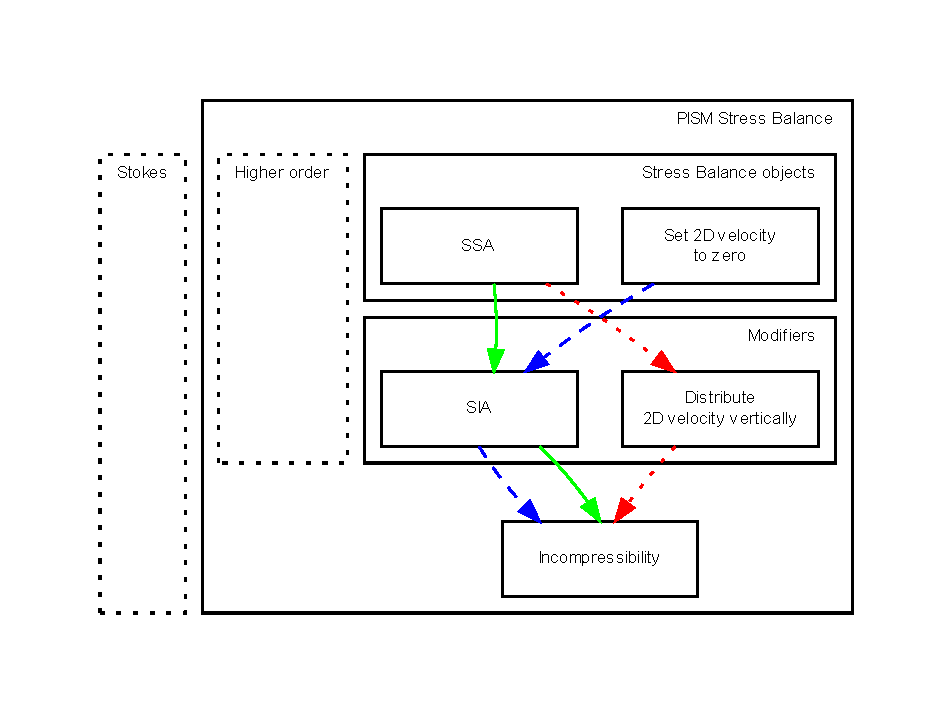
\includegraphics[width=6in]{stressbalance}
  \caption{The SIA-only, SSA-only, and SIA+SSA hybrid models represent different ``routes'' through stress balance PISM components.  In each case the inputs are ice geometry and boundary stresses, and the final output is a three-dimensional velocity field within the ice.}
  \label{fig:stressbalance}
\end{figure}


\subsection{Climate inputs, and their interface with ice dynamics}
\label{sec:climate-inputs}  

Because PISM's job is to approximate ice flow, its ``world view'' is centered around ice dynamics.  The discussion of boundary conditions, in this \emph{Manual} is necessarily ``ice-centric'' in our description here, but there is no constraint on the nature of, or completeness of, climate models which could be coupled to PISM.  This section applies the PISM organizing principle above (section \ref{sec:dynamics}): \emph{climate inputs affect ice dynamics by a well-defined interface}.

Figure~\ref{fig:climate-inputs} illustrates that any PISM ice sheet model has an interface (green) to a surface processes layer containing snow, firn, and liquid (or refrozen) runoff, and to the ocean (blue) if there is floating ice.  The surface processes layer might be very simple.  If it is ``owned'' by the PISM model then there is an additional interface (red) to the atmosphere above.  The interface to the surface layer is assumed in PISM to cover the whole surface of the ice, including ablation areas and even ice-free land.  Table \ref{tab:ice-dynamics-bc} lists fields which are needed as boundary conditions at the interfaces.

\begin{figure}
  \centering
  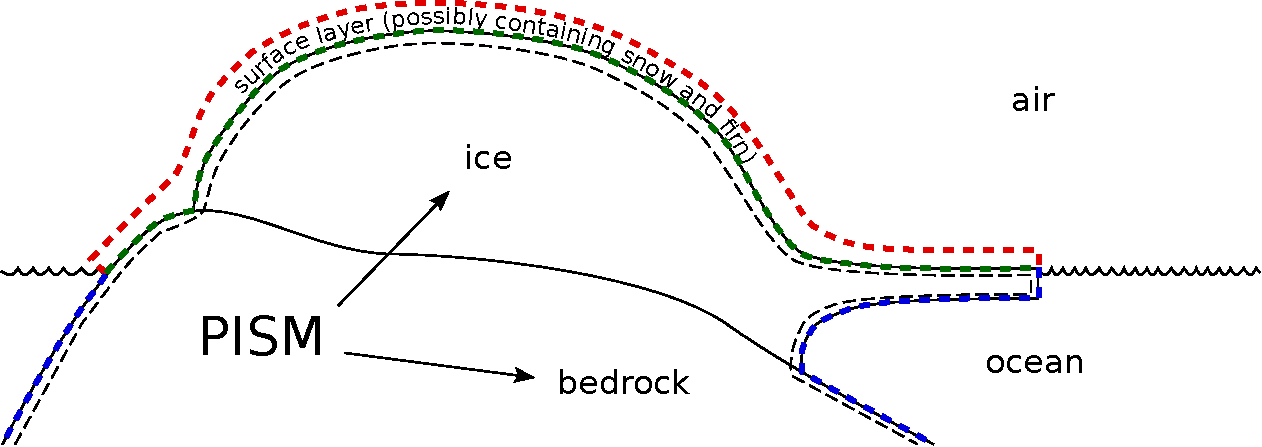
\includegraphics[width=6in]{figs/climate-cartoon.pdf}
  \caption{PISM's view of interfaces between an ice sheet and the outside world}
  \label{fig:climate-inputs}
\end{figure}

\begin{table}[h]
  \centering
 \begin{tabular}{p{0.35\linewidth}p{0.55\linewidth}}
    \toprule
    \textbf{Boundary} & \textbf{Necessary conditions}\\
    \midrule
    Top ice surface (below firn) (\textcolor{green}{green})& Ice temperature (or enthalpy) and mass flux into the ice\\
    Bottom surface of the thermal bed layer (not shown) & Geothermal flux\\
    Ice shelf basal surface (\textcolor{blue}{blue})& Mass flux into the ocean and ice boundary temperature\\
   \bottomrule
  \end{tabular}
\caption{Boundary conditions required by PISM's ice dynamics core; see figure \ref{fig:climate-inputs}}
\label{tab:ice-dynamics-bc}
\end{table}

Regarding the base of the ice, as described in section \ref{subsect:beddef} PISM also includes an optional bed deformation component approximating the movement of the Earth's crust and upper mantle in response to changing ice load.   Furthermore the temperature of the layer of bedrock in contact with grounded ice is included in the conservation of energy model.  In this sense everything below the black dashed line (i.e.~ice and bedrock) is ``owned'' by PISM.  This fact adds two more boundary interfaces for the ice dynamics core: sub-ice-shelf/ocean (shown in blue) and the bottom of the bedrock thermal layer (not shown).

The PISM ice dynamics core would like to be able to get fields listed in Table
\ref{tab:ice-dynamics-bc} directly from observations or measurements, or directly from a GCM.  In many realistic modeling situations, however, PISM code must be used for all or part of the surface processes modeling necessary to provide the ice-dynamics core with the ``right'' fields.  Due to differences in model resolutions and required down-scaling, this need for some PISM-based boundary-processes modeling includes cases where PISM is coupled to a GCM.  In the kind of ``offline'' runs described in this \emph{Manual}, boundary processes are modeled, even if trivially.

Thus, to be able to use the data that \emph{is} available, an ice-sheet model has to
have additional components that are responsible for modeling surface (snow)
processes or sub-shelf/ocean interaction.  These components might be very minimal, merely turning data that we already have into data in the right units and with the right metadata, so that PISM knows what to do with it, for example.

Thus we have PISM's design: the ice-dynamics-and-earth-deformation PISM
core does not contain any parameterization or other model for boundary mass or
energy balance.  These boundary parameterizations and models are present in the PISM source code, however, as instances of \emph{PISMComponent} classes.  This simplifies customizing and debugging PISM's climate
inputs, promotes code reuse.  Moreover, it isolates the code that needs to be changed to
couple PISM to a climate model.

Users wishing to customize PISM's climate inputs should see the \emph{PISM
  Source Browser} at
\begin{quote}
  \url{\PISMBROWSERURL}
\end{quote}
 and the documentation
of \mbox{\emph{PISMSurfaceModel}}, \mbox{\emph{PISMAtmosphereModel}}, and
\mbox{\emph{PISMOceanModel}} therein.  Also, section \ref{sec:start} describes a
modeling example using a non-standard air temperature parameterization. Looking
at the file
\begin{quote}
\texttt{src/coupler/atmosphere/PAEismintGreenland.cc}
\end{quote}
may be a reasonable start.

Note that figure~\ref{fig:climate-inputs} includes an interface between the surface layer and the air (red dashed line).
Unlike the ones listed in table~\ref{tab:ice-dynamics-bc}, this interface
\emph{may not even be present in some PISM configurations:} the ice dynamics
core of PISM only ``knows'' about mediums bordering ice and bedrock. A pair
consisting of a \emph{PISMSurfaceModel} and a \emph{PISMOceanModel} may be
hiding anything from a nearly trivial parameterization of ice surface
temperature plus surface and sub-shelf mass fluxes to a GCM of great
complexity.

Figure~\ref{fig:climate-input-data-flow} illustrates the corresponding data
flow \emph{into} the PISM core; the data flow in the other direction depends on
particular modeling choices.

This figure requires an explanation: a ``modifier'' in this context is an
adjustment of climate inputs that can be used with different climate
choices.  Using ice-core-derived air temperature offsets to model the
space-time distribution of paleo surface temperature is an example.  Note that
PISM has a generic ``forcing'' mechanism that can be paired with another model.
Please see the \emph{PISM's climate forcing components} document for
a list of climate components included in PISM source code and other details.

\begin{figure}
  \centering
  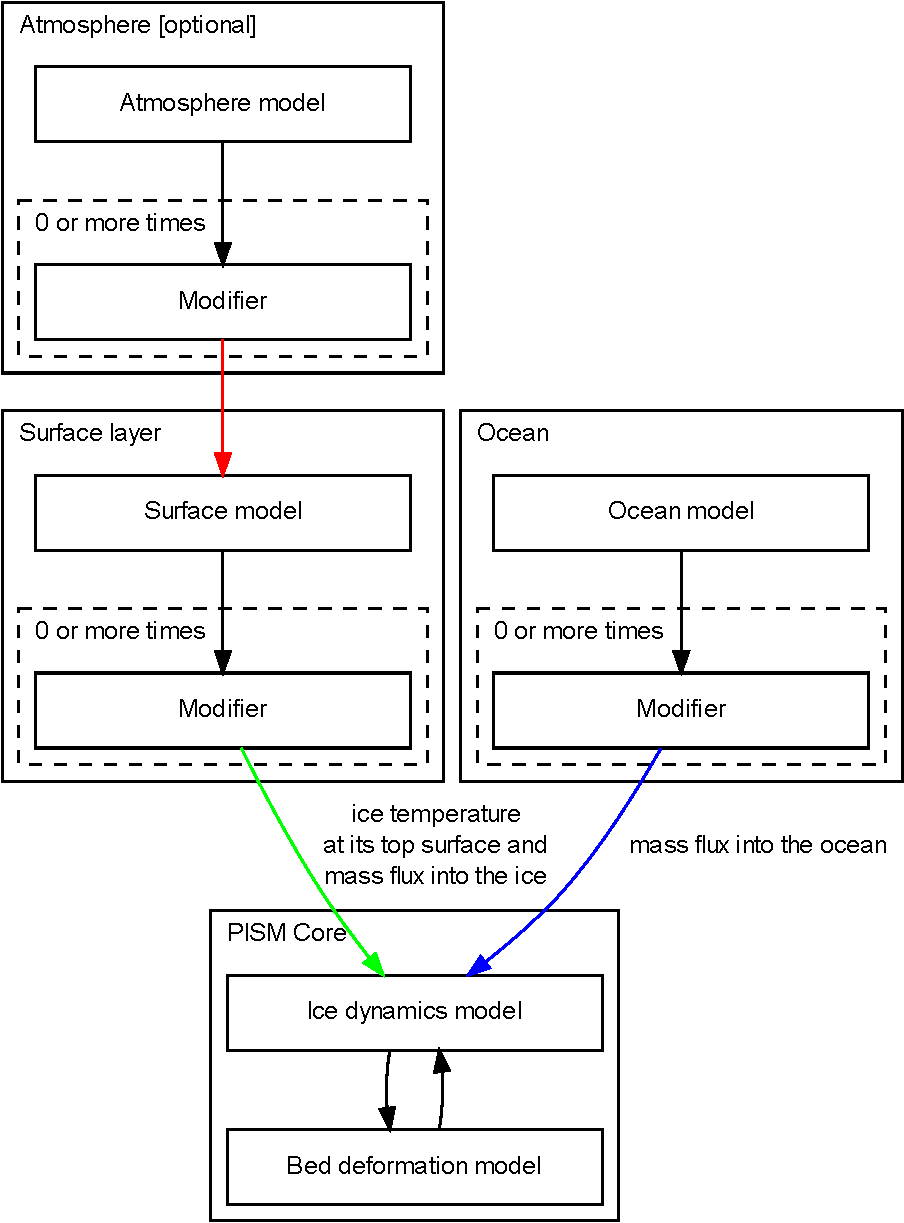
\includegraphics[width=5in]{figs/data-flow.pdf}
  \caption{PISM climate input data flow. Colored arrows correspond to interfaces in
    Figure \ref{fig:climate-inputs}.}
  \label{fig:climate-input-data-flow}
\end{figure}

Why describe this structure here? On the one hand, some users may be interested
in coupling PISM to other models. On the other hand, the PISM authors do not
claim expertise in modeling atmosphere, ocean, or even snow processes.   So the
separation has a code-reliability purpose. Indeed PISM users need to know that
they are ultimately responsible for providing the climate inputs they intend.

\clearpage
\newpage
\section{Initialization and bootstrapping}
\label{sec:boot}

There are three ways to start PISM,\begin{itemize}
\item \texttt{-i} reads a previously-saved PISM model state, a NetCDF file,
\item \texttt{-boot_file} reads an ``incomplete'' NetCDF file and uses heuristics to fill in needed fields, and
\item the executables \texttt{pisms} and \texttt{pismv} initialize simplified-geometry experiments and verification tests, respectively, from formulas in the source code.
\end{itemize}

Realistic modeling usually starts with the \texttt{-boot_file} option because real ice sheet observations are never complete initial conditions for ice sheet models.  Runs with multiple stages generally use the \texttt{-i} option after the first stage.

\subsection{Initialization from a saved model state}  ``Initialization''\index{initialization!from saved model state} has the specific, simple meaning in PISM that option ``\texttt{-i}'' was used.  If a previous PISM run has saved a NetCDF file using ``\texttt{-o}'' then that file will contain complete initial conditions for continuing the run.  The output file from the last run can be loaded with ``\texttt{-i}'': \index{executables!\texttt{pisms}}

\begin{verbatim}
$ pisms -eisII A -y 100 -o foo.nc
$ pisms -eisII A -i foo.nc -y 100 -o bar.nc
\end{verbatim}
\smallskip

Note that simplified-geometry experiments (section \ref{sec:simp}) and verification tests (section \ref{sec:verif}) do not need input files at all because they initialize from formulas in the source code.  They can be continued from saved model states using \texttt{-i}.

In the above example, specifying the simplified geometry experiment or verification test \emph{is} necessary if the run is to continue with the climate inputs for that experiment or test.  For example, based on the above \texttt{pisms} runs, it is valid to do
\begin{verbatim}
$ pismr -i foo.nc -y 100 -o bar.nc
\end{verbatim}
but the climate and other parameters use PISM default values, and thus are not (necessarily) the values specified in EISMINT II.

As a technical but important note about saved states, a PISM run with \texttt{-ssa_floating_only} or \texttt{-ssa_sliding}
also saves the last SSA velocities to the output file, in variables 
\texttt{u_ssa} and \texttt{v_ssa}.  The presence
of these velocities adds efficiency in restarting because a initial estimate speeds up the solution of the stress balance equations.  If you want a PISM restart to
ignore these velocities use \texttt{-dontreadSSAvels}.

\subsubsection*{\texttt{-i} file format}
\label{sec:i-format}
PISM produces\footnote{Or, more accurately, attempts to produce; please let us know about violations you come across.} CF-1.5 compliant NetCDF\index{PISM!NetCDF file format}\index{NetCDF} files.  The easiest way to learn the output format \emph{and} the \texttt{-i} format is to do a simple run and then look at the metadata in the resulting file, like this:
\begin{verbatim}
$ pisms -eisII A -y 10 -o foo.nc
$ ncdump -h foo.nc | less
\end{verbatim}

Note that variables have a \texttt{pism_intent}\index{PISM!\texttt{pism_intent} attribute} attribute.  When that attribute is \texttt{diagnostic}, the variable can be deleted from the file without affecting whether PISM can use it as a \texttt{-i} input file.  Variables with \texttt{pism_intent} = \texttt{model_state}, by contrast, must be present for use with \texttt{-i}.

The automatically produced \texttt{time} variable has a \texttt{units} attribute like \texttt{"seconds since 1-1-1"}.  Note that CF metadata conventions require using a reference date in the units string of a time (\texttt{time}) variable. By default PISM ignores this reference date, except when it is used in unit conversions based on a calendar (see below).


\subsection{Bootstrapping}
\label{sec:bootstrapping}
\optsection{Bootstrapping}
\optseealso{Grid}

``Bootstrapping''\index{bootstrapping}\index{initialization!by bootstrapping} in PISM means starting a modeling run with less than sufficient data, and letting the model fill in needed values according to heuristics.  These heuristics are applied before the first time step is taken, so they are part of an initialization process.  Bootstrapping uses the option \fileopt{boot_file}.

The need for an identified stage like ``bootstrapping'' comes from the fact that initial conditions, for the evolution equations describing an ice sheet, are not typically observable.  As a principal example of this problem, these equations require the temperature within the ice at the time the run is started.  Glaciological observations, specifically remote-sensed observations which cover a large fraction or all of an ice sheet, never include this temperature field in practice.

Instead, evolutionary ice sheet modeling necessarily does something like this
to get ``reasonable'' initial fields within the ice:
\begin{enumerate}
\item start only with (potentially) observable quantities like surface elevation, ice thickness, ice surface temperature, surface mass balance, and geothermal flux,
\item ``bootstrap'' as defined here, using heuristics to fill in temperatures at depth and to give a preliminary estimate of the basal sliding condition and the three-dimensional velocity field, and
\item \begin{enumerate}
      \item \emph{either} do a long run holding the current geometry and surface conditions steady, to evolve toward a steady state which has compatible temperature, stress, and velocity fields,
      \item \emph{or} do a long run using an additional (typically spatially-imprecise) historical record from an ice core or a sea bed core (or both), to apply forcing to the surface temperature or sea level (for instance), but with the same functional result of filling in temperature, stress, and velocity fields.
      \end{enumerate}
\end{enumerate}

When using \fileopt{boot_file} you will need to specify both grid dimensions (using \texttt{-Mx}, \texttt{-My} and \texttt{-Mz}) and the height of the computational box for the ice with \texttt{-Lz}.  The data read from the file can determine the horizontal extent of the model, if options \texttt{-Lx}, \texttt{-Ly} are not set.  The additional specification of vertical extent by \texttt{-Lz} is reasonably natural because typical data used in ``bootstrapping'' are two-dimensional.  Using \texttt{-boot_file} without specifying all four options \texttt{-Mx}, \texttt{-My}, \texttt{-Mz}, \texttt{-Lz} is an error.

If \texttt{-Lx} and \texttt{-Ly} specify horizontal grid dimensions smaller than in the bootstrapping file, PISM will cut out the center portion of the domain.  Alternatively, options \intextoption{x_range} and \intextoption{y_range} each take a list of two numbers, a list of minimum and maximum $x$ and $y$ coordinates, respectively (in meters), which makes it possible to select a subset that is not in the center of the bootstrapping file's grid.

For the key issue of what heuristic is used to determine the temperatures at depth, there are two methods.  The default method uses ice thickness, surface temperature, surface mass balance, and geothermal flux.  The temperature is set to the solution of a steady one-dimensional differential equation in which conduction and vertical advection balance, and the vertical velocity linearly interpolates between the surface mass balance rate at the top and zero at the bottom.  The non-default method, set with option \intextoption{boot_no_smb_in_temp}, was the default in older PISM versions (\texttt{stable0.5} and earlier); it does not use the surface mass balance and instead makes an even more heuristic estimate of the vertical profile which connects the surface temperature and basal (geothermal) flux boundary conditions.

\subsubsection*{\texttt{-boot_file} file format}
\label{sec:bootstrapping-format}

Allowed formats for a bootstrapping file are relatively simple to describe. 
\begin{enumerate}
\item NetCDF variables should have the \texttt{units} containing a
  UDUNITS-2-compatible string. If this attribute is missing, PISM will assume
  that a field uses MKS units.\footnote{PISM uses a library called UDUNITS-2\index{PISM!uses UDUNITS when reading NetCDF files}\index{UDUNITS-2} to convert data present in an input file to MKS.   This means that having ice thickness in feet or kilometers, or temperature in Celsius for example, is allowed.}
\item NetCDF coordinate variables should have \texttt{standard_name} or
  \texttt{axis} attributes. These are used to
  determine which \emph{spatial} dimension a NetCDF dimension corresponds to;
  please see a \texttt{ncdump -h} output from a file produced by PISM for an example. (This implies
  that \texttt{x} and \texttt{y} dimensions need not be called ``\texttt{x}''
  and ``\texttt{y}''.
\item Coordinate variables have to be strictly increasing.
\item All three-dimensional variables will be ignored in bootstrapping.
\item The \texttt{standard_name} attribute is used to identify a variable, so
  the variable names need not match corresponding variables in a
  PISM output file. Please see \url{\PISMBROWSERURL} for a list of CF standard
  names used in PISM.
\item Any two-dimensional variable except bed topography and ice thickness may
  be missing. For those missing variables some heuristic will be applied. See
  table \ref{tab:modelhierarchy} for a sketch of the data necessary for
  bootstrapping, and \texttt{src/base/iMbootstrap.cc} for all further details.
\item The bed elevation (topography) is read by \texttt{standard_name} =
  \texttt{bedrock_altitude} and the ice thickness by \texttt{standard_name} =
  \texttt{land_ice_thickness}.
\item Surface elevation is ignored if present. Users with surface elevation and
  bed elevation data should compute the ice thickness variable, put it in the
  bootstrapping file, and set its \texttt{standard_name} to \texttt{land_ice_thickness}.
\end{enumerate}
